\subsection{Eulerovské a úplné bipartitní podgrafy}


$G = (V,E)$ je souvislý graf. $V_G = \{$spanning\footnote{Česky též \uv{napnuté} --
podgrafy obsahující všechny vrcholy grafu $G$ (i kdyby některé z~nich byly
izolované).} podgrafy $G\}$

\tv $V_G$ je vektorový prostor nad $\GF(2)$, tedy místo sčítání podgrafů bereme jejich
symetrickou diferenci.

\begin{center}
	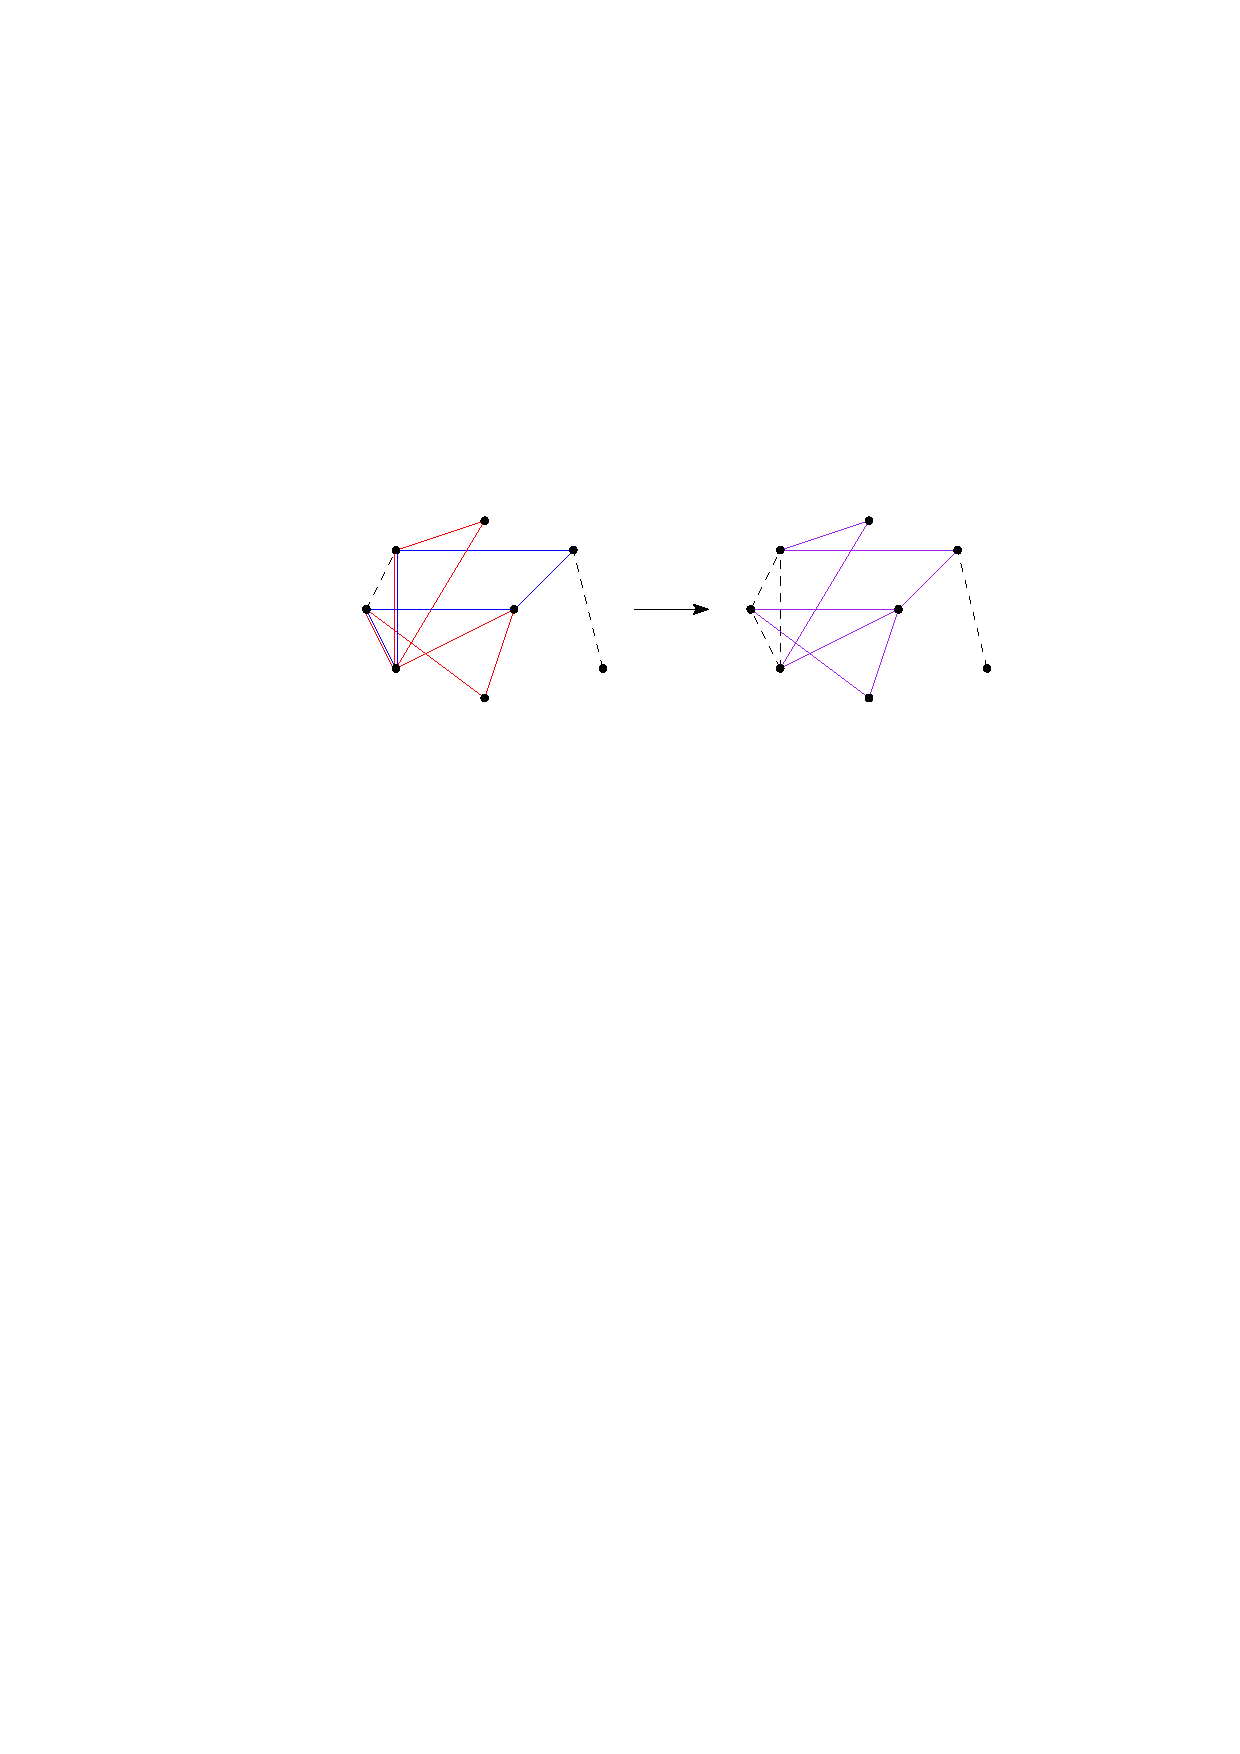
\includegraphics{symetricka_diference.pdf}
\end{center}

\df $\varepsilon_G = \{$eulerovské podgrafy $\equiv \forall $ stupně sudé$\}$. Součtem
dvou eulerovských podgrafů je eulerovský podgraf, tvoří tedy podprostor $V_G$.

\lm $\dim \varepsilon_G = |E| - n + 1$

\dk Vybereme si libovolnou kostru $T$ grafu $G$. Pro každou hranu, která není v~kostře
existuje právě jedna elementární kružnice $K_e$ určená touto hranou. $\{ K_e\ |\ e \in
E(G) - E(T) \}$ tvoří lineárně nezávislé vektory. Navíc tvoří bázi $\varepsilon_G$ ($H
= \oplus \left\{ K_e \mid e \in E(L) \setminus E(T) \right\}$ pro daný eulerovský graf
$L$, $H \oplus L$ je mimo kostru nulová a navíc víme, že je eulerovským podgrafem
kostry, tedy prázdným podgrafem a tudíž máme jejich rovnost).

Z~toho $\dim \varepsilon_G = |E| - n + 1$, což je počet hran mimo kostru. \qed

\df $\beta_G = \{$úplné bipartitní spanning podgrafy $G\}$. $\beta_G$ je
prostor všech řezů v~$G$.

\lm $\beta_G \ll V_G$, $\beta_G = \langle\{$ hvězdy $\}\rangle$

\dk Každý úplný bipartitní podgraf lze zapsat jako symetrickou diferenci hvězd.
Vezmeme hvězdy ze všech vrcholů v~jedné z~partit. Mezi těmito vrcholy se hrany
vyruší, mezi vrcholy z~druhé partity žádné nevedou a všude jinde ano. 

Mám-li dva různé úplné bipartitní podgrafy, rozepíšu si je na součet hvězd a
výsledkem musí být dle výše uvedeného opět úplný bipartitní podgraf.

\vt $\varepsilon_G^\bot = \beta_G$. Tedy eulerovské podgrafy jsou ortogonálním
doplňkem úplných bipartitních podgrafů.

\dk Vezmeme si $H \in \varepsilon_G$ eulerovský podgraf a $u \in V(G)$. $H_u$
označíme hvězdu z~vrcholu $u$. Platí $\sk{H,H_u} = \deg_H u$, neboť hvězda
obsahuje všechny hrany jdoucí z~$u$ a žádné jiné. Protože v~$H$ vychází
z~každého vrcholu sudý počet hran a počítáme nad $\GF(2)$:
\begin{align*}
\forall u: \sk{H,H_u} = 0 \quad\Rightarrow\quad \forall B\in \beta_G: \sk{H,B} = 0 \quad\Rightarrow\quad H \in \beta_G^\bot \quad\Rightarrow\quad \varepsilon_G \subseteq \beta_G^\bot
\end{align*}

Naopak, každý podgraf $H$, který je kolmý na všechny hvězdy je nutně eulerovský:
\begin{align*}
\forall u: \sk{H,H_u} = 0 \quad\Rightarrow\quad \forall u: \deg_H u~\equiv 0 \mod 2 \quad\Rightarrow\quad H \in \varepsilon_G \quad\Rightarrow\quad \beta_G^\bot \subseteq \varepsilon_G
\end{align*}

Tedy $\varepsilon_G = \beta_G^\bot$, protože $\varepsilon_B^\bot = {\left(\beta_G^\bot\right)}^\bot = \beta_G$.
\qed

\dsl $\dim \varepsilon_G = \dim \beta_G^\bot = |E| - n + 1$.


\vt $M \subseteq \GF(2)^n \quad\Rightarrow\quad (1,1,\dots,1) \in \sk M + M^\bot = \sk{M\cup M^\bot}$

\dk $\sk M \cap M^\bot$
\begin{enumerate}
\item[(a)] $\dim(\sk M \cap M^\bot) = 0 \quad\Rightarrow\quad \dim(\sk M + M^\bot) = k+n-k = n \Rightarrow \sk M + M^\bot = \GF(2)^n \Rightarrow (1,1,\dots,1)\in \sk M + M^\bot$
\item[(b)] $\dim(\sk M \cap M^\bot) > 0 \quad\Rightarrow\quad \exists u\in \sk M \cap M^\bot$ \\ 
$\forall u\in \sk M \cap M^\bot: \sk{u,u} = 0 \Rightarrow \sum u_i^2 \equiv 0 \mod 2 \Rightarrow \sum u_i = \sk{u, (1,1,\dots,1)}$ \\
nad $\GF(2)$ platí $u_i^2 = u_i$ \\
$\Rightarrow (1,1,\dots,1) \in {(\sk M \cap M^\bot)}^\bot = {\sk M}^\bot + {(M^\bot)}^\bot = M^\bot + \sk M$
\end{enumerate}
\qed


\vt $\forall G \ \exists V_1,V_2,\ V_1\overset{.}{\cup} V_2 = V(G)$ takové, že
$G[V_1]$ i $G[V_2]$ mají všechny stupně sudé.

\dk $M = \varepsilon_G \ll V_G$

$G = (1,1,\dots,1) \in \varepsilon_G + \varepsilon_G^\bot = \varepsilon_G + \beta_G$
\qed

\dsl $\exists H \in \varepsilon_G\ \exists B\in \beta_G: G = H + B$ (tedy každý graf lze zapsat jako symetrickou diferenci eulerovského podgrafu a hranového řezu).


